\scanpage{140}
\deleted{$H^i(C,$}
\[
\underline H^i_{U/k}(F)\qquad\operatorname{Ext}^i
\]
\[
\underline{\operatorname{Ext}}^i_{U/k}(G,\widetilde{\unsure{\sigma|\tau}})\simeq
\underline{\operatorname{Ext}}^i_k(N_f^{\unsure{\bullet|'}}(G),\unsure{\sigma|\tau})
\]
\diagram{\begin{tikzcd}[column sep=large,row sep=large]
\underline{\operatorname{Ext}}^i_{\unsure{C|S}/K}(G,\widetilde{\unsure{\sigma|\tau}})\arrow[d]&\underline{\operatorname{Ext}}^i_k(N^{\unsure{\bullet|'}}(G),\unsure{\sigma|\tau})\\
\underline{\operatorname{Ext}}^i_{U/k}(G,\widetilde{\unsure{\sigma|\tau}})&\underline{\operatorname{Ext}}^i_k(N^{\unsure{\bullet|'}}(G_U),\unsure{\sigma|\tau})\arrow[u]
\end{tikzcd}}
\diagram{\begin{tikzcd}
0\arrow[r,dash]&G_U\arrow[r,dash]&G\arrow[r,dash]&G^Y\arrow[r,dash]&0
\end{tikzcd}}
\figure{
\begin{tikzpicture}[x=1cm,y=1cm]
\draw[gray,rotate=50] (0,0) ellipse (.6 and .22);
\draw[gray](-.5,-.1)..controls(-.2,.6)and(.6,.7)..(.6,.2)..controls(.6,-.2)and(-.2,-.4)..(-.45,-.25);
\draw[gray](.4,-.5)--(.35,1);
\draw[gray](.8,-.7)--(.8,.6);
\draw[gray](1.5,-.6)--(1.1,.15)--(1.7,-.4)--(1.7,.15);
\draw[gray](.3,-.8)--(1.8,.45);
\draw[gray](.5,-.9)--(1.9,.35);
\draw[gray](.2,-.65)--(1.8,.4);
\draw[gray](.7,-.85)--(1.65,-.1);
\draw[gray](.9,-.95)--(1.9,-.1);
\end{tikzpicture}}
\diagram{\begin{tikzcd}[column sep=tiny,row sep=small]
\underline{\operatorname{Ext}}^*_{U/k}(G,\widetilde{\unsure{\sigma|\tau}})\arrow[d,equal]&=&\underline{\operatorname{Ext}}^*_{S/k}(G_U,\widetilde{\unsure{\sigma|\tau}})&=&\underline{\operatorname{Ext}}^*_k(N^{\unsure{\bullet|'}}_{\unsure{*|x}}(i_!(G)),\unsure{\sigma|\tau})\\
\underline H^*_{U/k}(\widehat G)&&\Vert&&\\
&&i_!(G_{\unsure{\infty|U}})&&
\end{tikzcd}}
\figure{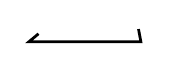
\begin{tikzpicture}[x=1cm,y=1cm]\draw[line width=1pt](0,.1)--(-.12,0)--(1.3,0)--(1.27,.16);\end{tikzpicture}}
\[
\boxed{\underline H^*_{Y/k}(i_!(G))\overset{?}{\simeq}\underline H^*_{U/k}(G)}\qquad???
\]
\[
\underline H^*_{Y/k}(i_!(G))\simeq\unsure{H|\vdash}
\]
\mspage{139}

